\documentclass{article}
\usepackage[utf8]{inputenc}
\usepackage{cmap}
\usepackage[T2A]{fontenc}
\usepackage[english,russian]{babel}
\usepackage{amsmath,amsfonts,amssymb,amsthm,mathtools}
\usepackage{graphics}
\title{Диффузия}
\author{Шмаков Владимир Евгеньевич}
\date{МФТИ, Март 2022}
\title{Исследование взаимной диффузии газов}

\begin{document}
	
\maketitle
\newpage
\section{Цель работы}
Рассчитать коэффициент взаимной диффузии бинарной смеси. Узнать о границах применимости закона Фика. Оценить длину свободного пробега атомов гелия при различных условаиях.
\section{Оборудование}
В работе используются сосуды объёмами $V_1=V_2=1200 cm^3$, система подачи газов, формваакумный насос, датчики теплопроводности, мост Уинстона.
\section{Обработка результатов эксперимента}
\subsection{Вычисление коэфициента взаимной диффузии}
Убедимся, что процесс подчиняется закону: \[\Delta{n} = \Delta{n_0}\exp\left(-\frac{t}{\tau}\right) \]
Для построим графики зависимости напряжения от времени, и по оси y выберем логарифмический масштаб:
\begin{figure}[h]
    \centering
    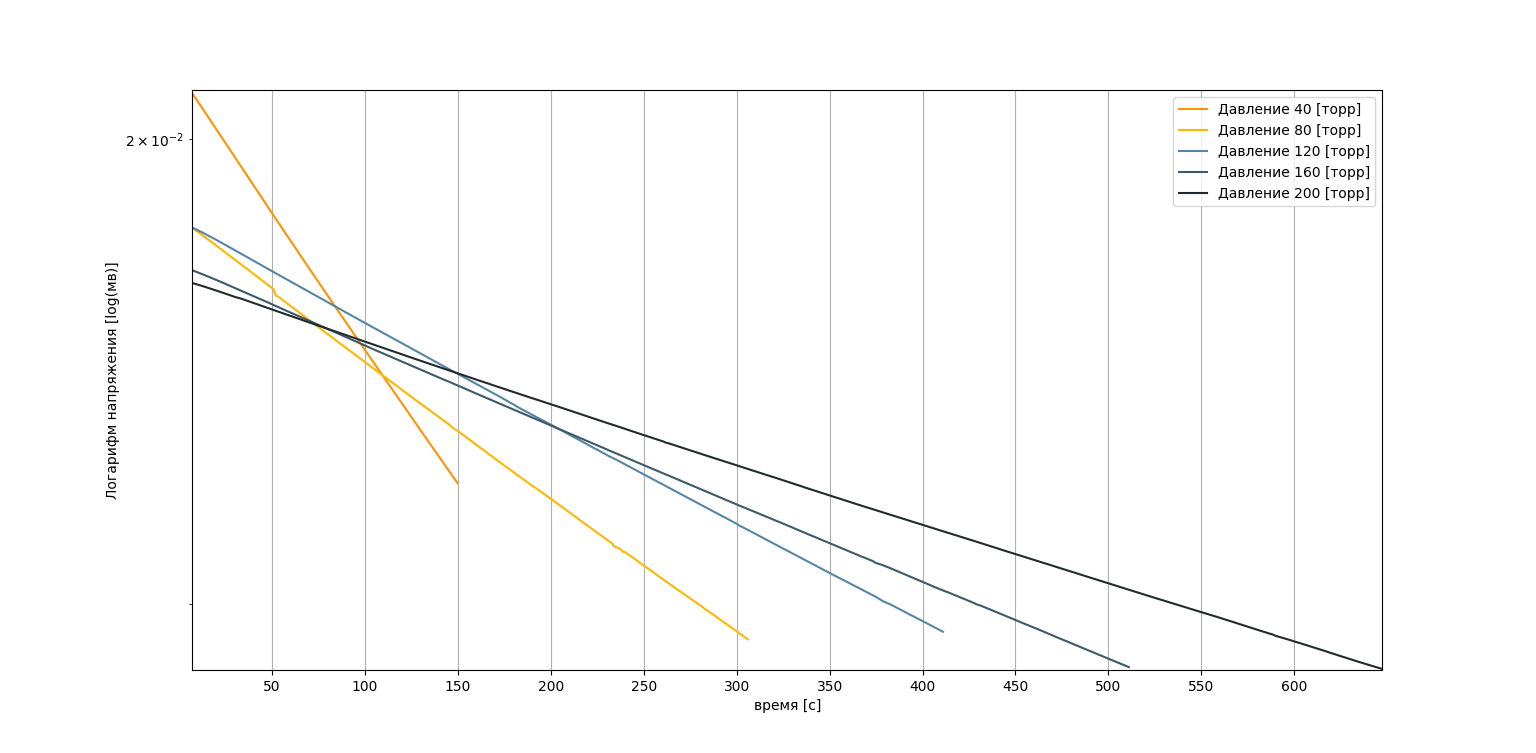
\includegraphics[scale = 0.3]{log(u)byT.png}
    \caption{Зависимость напряжения от времени}
    \label{fig:my_label}
\end{figure}

\newpage
Методом наименьших квадратов вычислим коэффициенты наклона прямых, и по формуле $U = U_0exp(-t/\tau)$ найдем характерное время процесса. Получим результаты:
\begin{table}[h]
    \centering
    \begin{tabular}{|c|c|c|}
        \hline
        \textbf{Номер эксперимента} & \textbf{Коэффициент наклона} & \textbf{Время процесса}\\
        \hline
        1 & $a_1 = -0.0047 \pm 4 \cdot 10^{-6}$ & $\tau_{1} = 213.3 \pm 0.2 \text{с}$ \\
        \hline
        2 & $a_2 = -0.0024 \pm 3 \cdot 10^{-6}$ & $\tau_{2} = 423.8 \pm 0.5 \text{с}$ \\
        \hline
        3 & $a_3 = -0.0017 \pm 1 \cdot 10^{-8}$ & $\tau_{3} = 580.9 \pm 0.3 \text{с}$ \\
        \hline
        4 & $a_4 = -0.0013 \pm 7 \cdot 10^{-7}$ & $\tau_{4} = 739.8 \pm 0.4 \text{с}$ \\
        \hline
        5 & $a_5 = -0.001 \pm 7 \cdot 10^{-7}$  & $\tau_{5} = 969.0 \pm 0.7 \text{с}$ \\
        \hline
    \end{tabular}
    \caption{Вычисление угловых коэффициентов и характерного времени процесса}
    \label{tab:my_label}
\end{table}
    

Зная характерное время процесса можем вычислить занчение коэффициента диффузии при данных условиях:
\begin{equation}\label{diffusion}
D = \frac{V L}{2 \tau S}
\end{equation}
Методом частных производных оценим погрешности вычислений:
\begin{equation*}
    \sigma_{V} = \Delta{V} \cdot \frac{\partial{D}}{\partial{V}} = \Delta{V} \cdot \frac{D}{V}
\end{equation*}
\begin{equation*}
    \sigma_{\tau} = \Delta{\tau} \cdot \frac{\partial{D}}{\partial{\tau}} = \Delta{\tau} \cdot \frac{D}{\tau}
\end{equation*}
\begin{equation*}
    \frac{L}{S} = \Delta{\frac{L}{S}} \cdot \frac{\partial{D}}{\partial{\frac{L}{S}}} = \Delta{\frac{L}{S}} \cdot \frac{D S}{L}
\end{equation*}
\begin{equation*}
    \sigma = \sqrt{\sigma_{\frac{L}{S}}^2+\sigma_{\tau}^2+\sigma_{V}^2}
\end{equation*}
В результате получим:
\begin{table}[h]
    \centering
    \begin{tabular}{l r}
        $P_1 = 40 \text{торр} $ & $D_1 = 1.5 \cdot 10^{-3} \pm 1 \cdot 10^{-4} \frac{\text{м}^2}{\text{с}}$ \\
        \\
        $P_2 = 80 \text{торр} $ & $D_2 = 7.8 \cdot 10^{-4} \pm 7 \cdot 10^{-5} \frac{\text{м}^2}{\text{с}}$ \\
        \\
        $P_3 = 120 \text{торр} $ & $D_3 = 5.6 \cdot 10^{-4} \pm 5 \cdot 10^{-5} \frac{\text{м}^2}{\text{с}}$ \\
        \\
        $P_4 = 160 \text{торр} $ & $D_4 = 4.5 \cdot 10^{-4} \pm 4 \cdot 10^{-5} \frac{\text{м}^2}{\text{с}}$ \\
        \\
        $P_5 = 200 \text{торр} $ & $D_5 = 3.4 \cdot 10^{-4} \pm 3 \cdot 10^{-5} \frac{\text{м}^2}{\text{с}}$ \\
    \end{tabular}
\end{table}
\newpage
Убедимся в линейной зависимости коэффициента взаимной диффузии от обратного давления, для этого по оси $x$ отложим значение $1/P$, а по оси $y$ соответвуюшее значение коэффициента взаимной диффузии $D$:
\begin{figure}[h]
\centering
    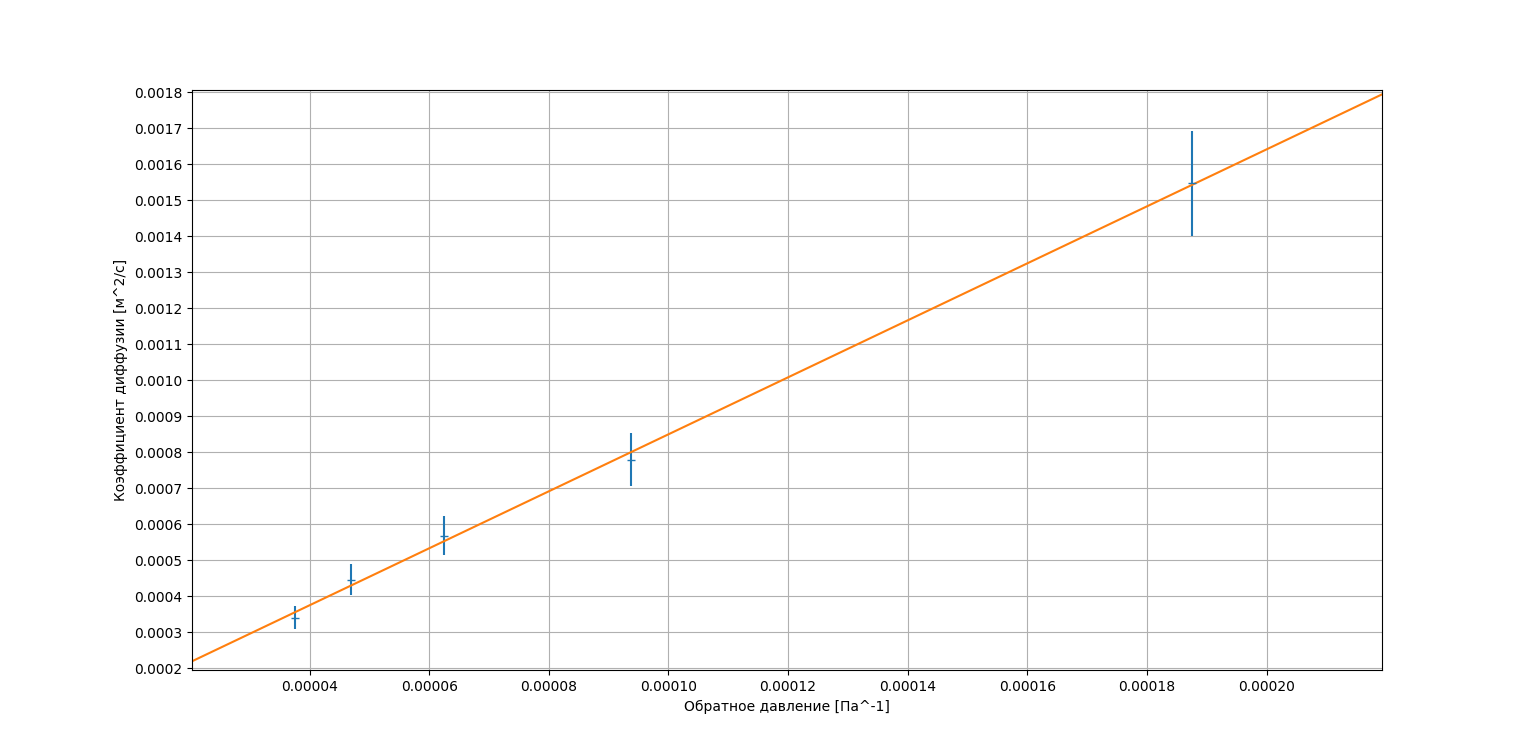
\includegraphics[scale = 0.3]{DbyinversedPressure.png}
    \caption{Зависимость коэффициента взаимной диффузии от обратного давления}
    \label{Dbyinversed Pressure}
\end{figure}
\subsection{Вычисление длины свободного пробега}
Длина свободного пробега атомов гелия может быть вычислена по формуле:
\begin{equation}\label{length}
\lambda = \frac{3 D}{\bar{u}}
\end{equation}
Где $\bar{u}$ - средняя тепловая скорость. Считаем температуру неизменной на протяжении всего эксперемента $T = 293 \pm 1 \text{K}$. Концентрация гелия в работе гораздо меньше концентрации воздуха $n_{He} \ll n_{\text{Возд}} $, кроме того атомы гелия существенно легче молекул составляющих воздух $\mu_{He} \ll \mu_{O_2}$, $\mu_{He} \ll \mu_{N_2}$. Поэтому перемешивание газов в работе можно приближенно описывать как диффузию примеси лёгких частиц He на практически стационарном фоне воздуха.

Найдем среднюю тепловую скорость частиц гелия:
\begin{equation*}
    \bar{u} = \sqrt{\frac{8 R T}{\pi \mu_{He}}}
\end{equation*}

Оценим погрешность:
\begin{equation*}
    \sigma = \Delta{T} \cdot \frac{1}{2}  \sqrt{\frac{8 R}{T \pi \mu_{He}}}
\end{equation*}
\newpage
По формуле \eqref{length} найдем длину свободного пробега в условиях эксперимента:
\begin{table}[h]
    \centering
    \begin{tabular}{l}
         $\lambda_{1} = 3.7 \cdot 10^{-6} \pm 4 \cdot 10^{-7} \text{м}$ \\
         $\lambda_{2} = 1.9 \cdot 10^{-6} \pm 2 \cdot 10^{-7} \text{м}$ \\
          $\lambda_{3} = 1.4 \cdot 10^{-6} \pm 1 \cdot 10^{-7} \text{м}$ \\
           $\lambda_{4} = 1.0 \cdot 10^{-6} \pm 1 \cdot 10^{-7} \text{м}$ \\
            $\lambda_{5} = 8.2 \cdot 10^{-7} \pm 8 \cdot 10^{-8} \text{м}$ \\
    \end{tabular}
    \caption{Длина свободного пробега в различных экспериментах}
    \label{lal}
\end{table}
\section{Вывод}

С точностью $8 \% $ удалось вычислить коэффициент взаимной диффузии газов. $D$ линейно зависит от обратного давления $1/P$, что обосновывается формулой \eqref{length}. Выразим $P$ как функцию $P = f(n_{He},n_{\text{возд}},T) = (n_{He}+n_{\text{возд}}) k T$, и получим, что $D$ пропорциональна $1/P$. Наибольший вклад в ошибку вычисления коэффицинта диффузии вносит систематичекая погрешность, связанная с физическими размерами установки -- обьемами сосудов, длиной и площадью сечения соединяющей трубки. Стоит отметить, что методика измерений, не позволяет вычисить коэффициент взаимной диффузии при равных концентрациях газов. В этом случае придется учитывать теплоемкости всей смеси, а не только воздуха. Также методика не подходит для экспериментов с разреженными газами, так как в таком случае невозможно измерить теплоемкость резистивными датчиками.

С точностью $10 \%$ удалось вычислить длину свободного пробега частиц гелия. Данная величина, как и коэффициент взаимной диффузии, убывает с ростом давления. Очевидно, ведь при низком давлении в ваакумных средах длина свободного пробега может быть порядка $10^{-1} - 10^{3} \text{м}$.
\end{document}
